%; whizzy paragraph -pdf xpdf -latex ./whizzypdfptex.sh
%; whizzy-paragraph "^\\\\begin{frame}\\|\\\\emtext"
% latex beamer presentation.
% platex, latex-beamer でコンパイルすることを想定。 

%     Tokyo Debian Meeting resources
%     Copyright (C) 2012 Junichi Uekawa
%     Copyright (C) 2011 Nobuhiro Iwamatsu

%     This program is free software; you can redistribute it and/or modify
%     it under the terms of the GNU General Public License as published by
%     the Free Software Foundation; either version 2 of the License, or
%     (at your option) any later version.

%     This program is distributed in the hope that it will be useful,
%     but WITHOUT ANY WARRANTY; without even the implied warreanty of
%     MERCHANTABILITY or FITNESS FOR A PARTICULAR PURPOSE.  See the
%     GNU General Public License for more details.

%     You should have received a copy of the GNU General Public License
%     along with this program; if not, write to the Free Software
%     Foundation, Inc., 51 Franklin St, Fifth Floor, Boston, MA  02110-1301 USA

\documentclass[cjk,dvipdfmx,12pt]{beamer}
\usetheme{Tokyo}
\usepackage{monthlypresentation}

%  preview (shell-command (concat "evince " (replace-regexp-in-string "tex$" "pdf"(buffer-file-name)) "&")) 
%  presentation (shell-command (concat "xpdf -fullscreen " (replace-regexp-in-string "tex$" "pdf"(buffer-file-name)) "&"))
%  presentation (shell-command (concat "evince " (replace-regexp-in-string "tex$" "pdf"(buffer-file-name)) "&"))

%http://www.naney.org/diki/dk/hyperref.html
%日本語EUC系環境の時
\AtBeginDvi{\special{pdf:tounicode EUC-UCS2}}
%シフトJIS系環境の時
%\AtBeginDvi{\special{pdf:tounicode 90ms-RKSJ-UCS2}}

\title{東京エリアDebian勉強会}
\subtitle{第86回 2012年3月度}
\author{岩松 信洋\\iwamatsu@debian.org\\Twitter: @iwamatsu}
\date{2012年3月17日}
\logo{
\includegraphics[width=8cm]{image200607/openlogo-light.eps}}

\begin{document}

\frame{\titlepage{}}

\section{Agenda}

\begin{frame}{Agenda}
\begin{itemize}
\item 最近あったDebian関連のイベント報告
	\begin{itemize}
        \item 第85回 東京エリアDebian勉強会
        \item 第0回 福岡Debian勉強会
	\end{itemize}
\item Debian 勉強会 -ユーザサイド- Apache2 HTTP サーバから始めるDebian
\item 今後のイベント
\end{itemize}
\end{frame}


\emtext{自己紹介}

\begin{frame}{自己紹介}
\begin{itemize}
\item 岩松 信洋 (いわまつ のぶひろ) / @iwamatsu
\item Debian Project Official Developer
\item Bluetooth, OpenCV, mozc, libpng のメンテナ
\item 普段は Linux カーネル、ブートローダなどを開発
\item 「Gitによるバージョン管理」という本を書いたので買ってください
\end{itemize}
\end{frame}

\emtext{本日の資料}
\begin{frame}{本日の資料}

\begin{itemize}
\item セミナープレゼンテーション\\
\url{http://tokyodebian.alioth.debian.org/2012-03.html}
\item セミナーレジュメ
\url{http://tokyodebian.alioth.debian.org/2012-03.html}
\end{itemize}

全部メモを取る必要はありません。必要な事だけメモを取りましょう。

\end{frame}

\emtext{イベント報告}

\begin{frame}{第85回東京エリアDebian勉強会}
\begin{itemize}
\item Debian 開発者の為の KDE 開発環境について
\item 月刊Debhelper 第4回
\item cmake を使ってみた
\end{itemize}
\end{frame}

\begin{frame}{第0回福岡Debian勉強会}

\begin{itemize}
\item なぜか福岡に行ったので、勉強会をした。
\item DKMS の仕組みと Debian の対応状況
\item Debianサーバ量産工場 - 無限ポチポチ on Debian
\end{itemize}

\end{frame}

\emtext{Apache2 /HTTP サーバから始める Debian}

\section{Apache2 /HTTD サーバから始める Debian}

% [plain]
% [containsverbatim]
\begin{frame}[plain]

\begin{itemize}
\item 普段はちょっと開発者寄りな話をしている Debian 勉強会..\pause
\item Debian 勉強会は恐ろしい所!\pause ではない。\pause
\item 今回は OSC 出張企画として、ユーザー視点の勉強会を開催。\pause
\item ユーザサイド?ユーザ向けのDebian勉強会。\pause
\item ユーザの生の意見を取り入れ、Debian、Upsteamに反映(できるかも)。
\item 反応が良ければ次回もあるかもしれません。
\end{itemize}

\end{frame}

\begin{frame}
\begin{center}
\Huge{はじめに}
\end{center}
\end{frame}


\begin{frame}{はじめに}

\begin{itemize}
\item 噂によると、Debian は 世界(ヨーロッパ)でHTTPサーバとして一番採用されている Linux ディストリビューションらしい。\footnote{\url{http://w3techs.com/blog/entry/debian_is_now_the_most_popular_linux_distribution_on_web_servers}}\pause
\item 日本では HTTP サーバとしてあまり利用されているように見えませんが。

\end{itemize}

\end{frame}

\begin{frame}{はじめに}

\begin{itemize}
\item 利用されている理由は HTTP サーバパッケージの種類が多くある事が理由の一つだとか。
\item Apache HTTPD、Nginx、Lighttpd、etc..
\end{itemize}

\end{frame}

\begin{frame}{はじめに}

\begin{itemize}
\item 実際に利用している人(商業利用)に聞くと理由はこれだけではないようだ。\pause
\item Debianのパッケージングシステム\pause
\item APT\pause
\item Apahce モジュールパッケージの多さ \pause
\item Webアプリケーションで採用される P言語(Perl, Python, PHP)等のサポート\pause
\item {\color{red}設定ファイルの柔軟性}
\end{itemize}

\end{frame}


\begin{frame}{設定ファイルの柔軟性}

\begin{itemize}
\item Debian ってややこしいイメージ (らしい)\pause
\item Red Hat 系 と違い、Debian 特有の設定ファイルの構成 \pause
\item しかしなぜ特有の構成になっているのか? \pause
\item 理解すると、他のディストリビューションとのメリット、デメリットが見えてくるはず。
\end{itemize}

\end{frame}

\begin{frame}{はじめに}

というわけで今回は、Debian の Apache2 / HTTP サーバ (以下、Apache2 ) について勉強しましょう。

\end{frame}

\begin{frame}
\begin{center}
\Huge{Debian の Apache2\\バージョン}
\end{center}
\end{frame}

\begin{frame}{Debian の Apache2 バージョン}

\begin{center}
\begin{tabular}{|l|l|}
\hline 
ディストリビューション & バージョン \\
\hline \hline
stable & 2.2.16-6+squeeze6 \\
\hline
testing & 2.2.22-1 \\
\hline
unstable & 2.2.22-1 \\
\hline
experimental &  - \\
\hline
Upstream & 2.4.1 \\
\hline
\end{tabular}
\end{center}

\pause

\begin{itemize}
\item Upstream と比べると少し古いが、機能的には問題ない。
\item もちろんセキュリティアップデートにも対応。
\item RHEL、CentOS(\texttt{バージョン 2.2.15-15})と比べても特にバージョンが古いというわけでもない。
\end{itemize}

\end{frame}

\begin{frame}[plain]

\begin{center}
\Huge{Debian のパッケージ構成とパッケージのインストール}
\end{center}

\end{frame}

\begin{frame}{パッケージ構成}

\begin{center}
\begin{tabular}{|l|l|}
\hline 
パッケージ名 & パッケージの説明\\
\hline \hline 
apache2 & Apache HTTP サーバメタパッケージ \\
\hline
apache2-mpm-worker & スレッドモデル HTTP サーバ\\
\hline 
apache2-mpm-prefork & 非スレッドモデル HTTP サーバ\\ 
\hline
apache2-mpm-event & イベントドリブンモデル HTTP サーバ\\ 
\hline 
apache2-mpm-itk & マルチユーザ環境 HTTP サーバ\\
\hline
apache2.2-common & Apache HTTP サーバ 共通ファイル \\
\hline
apache2.2-bin & Apache HTTP サーバ 共通バイナリ\\ 
\hline
apache2-utils & ウェブサーバ用ユーティリティ \\
\hline
apache2-suexec & mod-suexec 用 基本 suexec \\
\hline
apache2-suexec-custom & mod-suexec 用 設定可能 suexec \\
\hline
apache2-doc & Apache HTTP サーバドキュメント \\
\hline
\end{tabular}
\end{center}

\end{frame}


\begin{frame}{パッケージ構成}

\begin{center}
\begin{tabular}{|l|p{16em}|}
\hline 
パッケージ名 & パッケージの説明\\
\hline \hline
apache2-dbg & Apache HTTP サーバ デバッグシンボルファイル \\
\hline
apache2-prefork-dev & 非スレッドモデル HTTP サーバ 開発用ファイル\\
\hline
apache2-threaded-dev & マルチスレッドモデル HTTP サーバ 開発用ファイル \\
\hline
\end{tabular}
\end{center}

\end{frame}

\begin{frame}{パッケージ構成}

\begin{itemize}
\item HTTP サーバの処理モデルごとにパッケージ
(apache2-mpm-worker、apache2-mpm-prefork、apache2-mpm-event、apache2-mpm-itk)
が分離されている。
\item 用途に合わせたパッケージをインストールできる。
\item Red Hat系は一つのパッケージに纏まっていて、処理モデル毎にサフィックスをつけている(例:httpd.worker)。
\end{itemize}

\end{frame}

\begin{frame}

\begin{center}
\Huge{パッケージ依存関係}
\end{center}

\end{frame}

\begin{frame}{パッケージ依存関係}

\begin{center}
  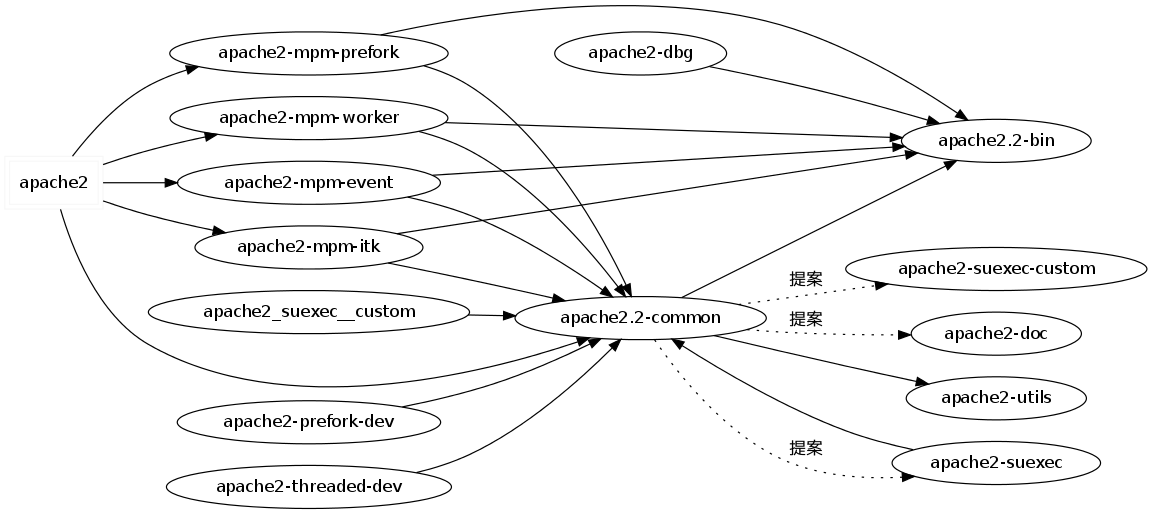
\includegraphics[width=1.0\hsize]{image201203/apache2-pkg.png}
\end{center}


\end{frame}

\begin{frame}{パッケージ依存関係}

\begin{itemize}
\item 依存関係が複雑なのでユーザは不安になるかもしれない。
\item Debianでは強力なパッケージ管理ツール APT によって気にする事なくインストールできる。
\end{itemize}

\end{frame}

\begin{frame}

\begin{center}
\Huge{インストール}
\end{center}

\end{frame}

\begin{frame}[containsverbatim]{インストール}

\begin{itemize}
\item Debianで パッケージをインストールする場合、 \texttt{apt-get install}コマンドを使う。
\item apache2 というメタパッケージを使ってインストールすることが多い。

\begin{commandline}
$ sudo apt-get update
$ sudo apt-get install apache2
\end{commandline}

\item デフォルトは apache2-mpm-worker(スレッドモデル HTTP サーバ)がインストールされる。
\item 他の HTTP サーバパッケージをインストールしたい場合は、各々のパッケージを
指定してインストールする必要がある。
\end{itemize}

\end{frame}

\begin{frame}{インストール}

\begin{itemize}
\item CentOSなどでは、「httpd」 パッケージとして提供されているのでパッケージ名が異なる。
\item 普段は他のディストリビューションを使っている人は注意すること。
\end{itemize}
\end{frame}

\begin{frame}

\begin{center}
\Huge{Apache HTTP サーバの起動と停止}
\end{center}

\end{frame}

\begin{frame}{Apache HTTP サーバの起動と停止}

\begin{itemize}
\item Debian は「インストールしたものは使う」というポリシー。\pause
\item パッケージインストール完了の時点で既に Apache HTTP サーバは起動している。\pause
\item 停止したい場合:\\
\texttt{sudo /etc/init.d/apache2 stop} \pause
\item 起動したい場合:\\
\texttt{sudo /etc/init.d/apache2 start} \pause
\item 再起動したい場合:\\
\texttt{sudo /etc/init.d/apache2 restart}
\end{itemize}

\end{frame}

\begin{frame}[containsverbatim]{Apache HTTP サーバの起動と停止}

\begin{commandline}
$ ps ax | grep apache2
10034 ?      Ss   0:05 /usr/sbin/apache2 -k start
13008 ?      S    0:00 /usr/sbin/apache2 -k start
....
$ sudo /etc/init.d/apache2 stop
$ ps ax | grep apache2
16833 pts/1  S+   0:00 grep apache2 
$ sudo /etc/init.d/apache2 start
$ ps ax | grep apache2
10048 ?      Ss   0:05 /usr/sbin/apache2 -k start
13024 ?      S    0:00 /usr/sbin/apache2 -k start
....
\end{commandline}
%$

\end{frame}

\begin{frame}{Apache HTTP サーバの起動と停止}

\begin{itemize}
\item デフォルトの状態では、マシンを立ち上げ時に HTTP サーバが起動するようになっている。\pause
\item 起動しないようにするには、ランレベル毎に動作するサーバ(サービス)変更する必要がある。\pause
\item サービスの起動設定 $\rightarrow$ \texttt{update-rc.d} コマンドを使う。
\end{itemize}

\end{frame}

\begin{frame}[containsverbatim]{Apache HTTP サーバの起動と停止}

\begin{itemize}
\item 全てのランレベルで Apache2 を起動させないように設定:\\
\texttt{sudo update-rc.d -f apache2 remove}

\item インストール直後のデフォルトの状態に戻したい場合:\\
\texttt{sudo update-rc.d -f apache2 default}
\end{itemize}

\end{frame}

\begin{frame}{Apache HTTP サーバの起動と停止}

\begin{itemize}
\item Red Hat系だと \texttt{chkconfig} を使う。\pause
\item Debian にはないんでしょ? \pause もちろんDebianでも提供されている。\pause
\item \texttt{chkconfig} は RedHat系のサービス管理ツールなので....。\pause
\item インターフェイスが似ている \texttt{sysv-rc-conf}があるのでこちらを使う。
\end{itemize}

\end{frame}


\begin{frame}[containsverbatim]{Apache HTTP サーバの起動と停止}

\begin{itemize}
\item 現在の状態を出力:\\
\texttt{sudo sysv-rc-conf --list}

\item ランレベル2のapache2を無効にする:\\
\texttt{sudo sysv-rc-conf --level 2 apache2 off}

\item ランレベル2のapache2を有効にする:\\
\texttt{sudo sysv-rc-conf --level 2 apache2 on}

\end{itemize}

\end{frame}


\begin{frame}[containsverbatim]{Apache HTTP サーバの起動と停止}

\begin{commandline}
$ sudo apt-get install sysv-rc-conf 
$ sudo sysv-rc-conf --list
apache2      0:off1:off2:on3:on4:on5:on6:off
bootlogd     S:on
(中略)
$ sudo sysv-rc-conf --level 2 apache2 off 
$ sudo sysv-rc-conf --list | head -1 
apache2      0:off1:off2:off3:off4:off5:off6:off
$ sudo sysv-rc-conf --level 2 apache2 on
$ sudo sysv-rc-conf --list | head -1
apache2      0:off1:off2:on3:off4:off5:off6:off
\end{commandline}
%$

\end{frame}

\begin{frame}
\begin{center}
\Huge{Apache2 の設定ファイル}
\end{center}
\end{frame}

\begin{frame}{Apache2 の設定ファイル}

\begin{itemize}
\item Red Hat 系の場合
\begin{itemize}
\item 主な設定は \texttt{/etc/httpd/conf/httpd.conf}で行う
\item include されるファイルは \texttt{/etc/httpd/conf.d/}ディレクトリに格納する。
\end{itemize}
\end{itemize}

\end{frame}

\begin{frame}{Apache2 の設定ファイル}

Debian の場合


\begin{center}
\begin{tabular}{|l|p{12em}|}
\hline 
設定ファイル & 内容\\
\hline \hline
/etc/apache2/apache2.conf & 基本設定\\
\hline
/etc/apache2/httpd.conf & オーバーライドする設定\\
\hline
/etc/apache2/conf.d/ & Includeするファイルを格納\\
\hline
/etc/apache2/ports.conf & ポートの設定\\
\hline
/etc/apache2/envvars & 環境変数の設定\\
\hline
/etc/apache2/mods-available/ & 利用可能なモジュール設定\\
\hline
/etc/apache2/mods-enabled/ & 利用中のモジュール設定\\
\hline
/etc/apache2/sites-available/ & 利用可能なサイト設定\\
\hline
/etc/apache2/sites-enabled/ & 利用中のサイト設定\\
\hline
/var/www & ドキュメントルート\\
\hline
/usr/lib/cgi-bin & cgi-bin\\
\hline
/var/log/apache2 & Apache2 ログ\\
\hline
\end{tabular}
\end{center}

\end{frame}



\begin{frame}[containsverbatim]{Apache2 の設定}
\begin{center}

\begin{center}
  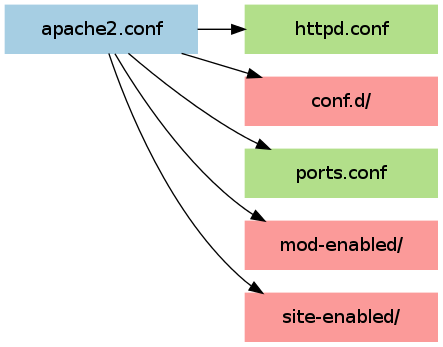
\includegraphics[width=0.9\hsize]{image201203/apache2-file.png}
\end{center}

\end{center}
\end{frame}

\begin{frame}[containsverbatim]{Apache2 の設定}

\begin{itemize}
\item \texttt{apache2.conf}には以下の行があり、\texttt{apache2.conf}
から各設定が読み込まれるようになっている。

\begin{commandline}
(省略)
# Include module configuration:
Include /etc/apache2/mods-enabled/*.load
Include /etc/apache2/mods-enabled/*.conf

# Include all the user configurations:
Include /etc/apache2/httpd.conf

# Include ports listing
Include /etc/apache2/ports.conf
(中略)
# Include generic snippets of statements
Include /etc/apache2/conf.d/

# Include the virtual host configurations:
Include /etc/apache2/sites-enabled/
\end{commandline}

\end{itemize}

\end{frame}


\begin{frame}{Apache2 の設定}

\begin{itemize}
\item Apache2 の設定を変更する場合、\texttt{apache2.conf}を変更しない。
\item \texttt{httpd.conf} や \texttt{ports.conf}を変更する。
\end{itemize}

\end{frame}


\begin{frame}
\begin{center}
\Huge{サイトの設定}
\end{center}
\end{frame}


\begin{frame}[containsverbatim]{サイトを設定する}

\begin{itemize}
\item Debian は\texttt{/etc/apache2/sites-available/default} に apache2 のデフォルトのサイト設定
を格納している。
\item サイトを一つだけ構築する場合はこのファイルを変更する。
\item 変更した後は、apache2 を再起動する。
\item 再起動方法\\

\begin{commandline}
$ sudo /etc/init.d/apache2 restart
\end{commandline}
%$

\end{itemize}
\end{frame}


\begin{frame}[containsverbatim]{サイトの設定}

\begin{itemize}
\item Debian の Apache2 で複数のサイトを立ち上げる場合、apache2.conf は編集しない。
\item サイト別に設定を記述し、\texttt{/etc/apache2/sites-available/}ディレクトリに格納する。
\item そのサイト設定を有効にするコマンド「\texttt{a2ensite}」実行し、Apache2 を再起動する。
\end{itemize}

\end{frame}

\begin{frame}[containsverbatim]{サイトの設定}


%\begin{commandline}
%
%<VirtualHost *>
%    ServerAdmin admin-test@example.org
%    ServerName test.example.org
%    DocumentRoot /home/test/public_html/
%    <Directory />
%        Options FollowSymLinks ExecCGI Includes
%        AllowOverride None
%    </Directory>
%</VirtualHost>
%\end{commandline}

\begin{enumerate}
\item サイト設定を記述する(test とする)。
\item サイト設定を\texttt{/etc/apache2/sites-available/test}に格納する。
\item \texttt{sudo a2ensite test}を実行する。\\
実行すると\texttt{/etc/apache2/sites-enabled/}
にシンボリックリンクが張られ設定が有効になる。
\item Apache2 を再起動する。\\
有効にしただけでは、稼働しているhttpd サーバには設定が反映されていないため。
\end{enumerate}

\end{frame}

\begin{frame}[containsverbatim]{サイトの設定}
\begin{commandline}
$ ls -F /etc/apache2/sites-enabled/
000-default@  default-ssl.old@
$ sudo a2ensite test
Enabling site test.
Run '/etc/init.d/apache2 reload' to activate new configuration!
$ ls -l /etc/apache2/sites-enabled/
000-default@  test@  default-ssl.old@
$ sudo /etc/init.d/apache2 restart
\end{commandline}

\end{frame}

\begin{frame}[containsverbatim]{サイトの設定を無効にする}

\begin{itemize}
\item サイトの設定を無効にする場合、「\texttt{a2dissite}コマンド」に無効にしたいサイトの設定ファイル名を指定して実行する。
\item 実行すると\texttt{/etc/apache2/sites-enabled/}からシンボリックリンクが削除される。
\item サイト設定を無効にした後は、有効時と同様に Apache2 を再起動する必要がある。
\end{itemize}

\begin{commandline}
$ sudo a2dissite test
Site test disabled.
Run '/etc/init.d/apache2 reload' to activate new configuration!
$ ls -l /etc/apache2/sites-enabled/ 
000-default@  default-ssl.old@
\end{commandline}
%$

\end{frame}

\begin{frame}[containsverbatim]{サイトの設定を無効にする}

\begin{itemize}
\item Debianではサイトの設定を分離し、サイト毎に状態を管理することができる。
\item 他のディストリビューションでは \texttt{include} 等を使って管理できるが、
ファイル内容を変更する必要があるので非常に手間。
\item Debian はシンボリックリンクを使うことによってApache2 の設定ファイルを
変更せずにサイト設定の有効・無効ができる。
\end{itemize}

\end{frame}


\begin{frame}
\begin{center}
\Huge{モジュールの設定}
\end{center}
\end{frame}


\begin{frame}[containsverbatim]{モジュールを有効/無効にする}

\begin{itemize}
\item  Debian のモジュールに関する設定はモジュール毎の設定ファイルとして
\texttt{mods-available}ディレクトリに格納されている。
\item それらのうち、実際に有効なものが \texttt{mods-enabled} ディレクトリにシンボリックリンクが張られる。
\item シンボリックリンクは手動で行わない。
\item モジュールを有効にする場合には\texttt{a2enmod}コマンドを使う。
\item 無効にする場合には\texttt{a2dismod}コマンドを使う。
\item 有効・無効にした後は Apache2 を再起動する。
\end{itemize}

\end{frame}

\begin{frame}[containsverbatim]{例: mod\_info を有効にする}

\begin{commandline}
$ ls -l /etc/apache2/mods-enabled/ | grep info 
(出力なし)
$ sudo a2enmod info
Enabling module info.
Run '/etc/init.d/apache2 restart' to activate new configuration!
$ sudo /etc/init.d/apache2 restart
.....
$ sudo /usr/sbin/apache2ctl -D DUMP_MODULES 2>/dev/null | grep info 
  info_module (shared)
\end{commandline}
%$

\end{frame}

\begin{frame}[containsverbatim]{例: mod\_info を無効にする}

\begin{commandline}
$ ls -l /etc/apache2/mods-enabled/ | grep info 
info.conf@
info.load@
$ sudo a2dismod info
Module info disabled.
Run '/etc/init.d/apache2 restart' to activate new configuration!
$ ls -l /etc/apache2/mods-enabled/ | grep info 
$ sudo '/etc/init.d/apache2 restart
.....
$ sudo /usr/sbin/apache2ctl -D DUMP_MODULES 2>/dev/null | grep info
(出力なし)
\end{commandline}
%$

\end{frame}


\begin{frame}{その他}

\begin{center}
\Huge{その他}
\end{center}

\end{frame}

\begin{frame}{libapache2-mod-php5 と apache2-mpm-prefork}

\begin{itemize}
\item apache2-mpm-worker(スレッドモデル) で PHP5(mod-php5) は使えない。
\item PHP5(mod-php5)の制限で、スレッドセーフではないため。
\item apache2-mpm-prefork (非スレッドモデル)を使う必要がある。
\item libapache2-mod-php5 をインストールすると、apache2-mpm-worker が削除され、apache2-mpm-prefork がインストールされる(親切設計)。
\item PHP ユーザの方は注意しましょう。
\end{itemize}
\end{frame}

\begin{frame}{再起動確認について}

\begin{itemize}
\item glibc が更新されたとき、サーバ系は再起動する必要がある。
\item Red Hat系では再起動してくれず、管理者が手動で行う必要がある。
\item CentOS を使っている会社ではデーモンを再起動しないとならないアップデートがあったかどうか
チェックするツールをわざわざ作って管理しているようだ。ダサイ。
\item しかし Debian では再起動の確認が行われる(設定によって自動再起動等も可能)。
\item 管理者の手を煩わせない。
\item このような細かいところに気を使ってくれるのも Debian の良い所。
\end{itemize}

\end{frame}

\begin{frame}{まとめ}

\begin{itemize}
\item Debian のパッケージ古いというのは昔の話。
\item セキュリティ対応あるし、早い。
\item Debian の設定ファイルが独自なのは理由がある。
\item 専用のツールもあるので、慣れるとメンテナンスが容易。
\item パッケージによる、細かいところへの気配り。
\item とりあえず、Debian 使え。
\end{itemize}

\end{frame}

\begin{frame}{質問}

\begin{center}
\Huge{何か質問はありますか?}
\end{center}

\end{frame}

\emtext{今後のイベント}
\begin{frame}{今後のイベント}
 \begin{itemize}
 \item 3月 関西 Debian 勉強会\\
   \begin{itemize}
     \item 第57回 関西 Debian 勉強会
     \item 日時: 2012 年 3 月 25 日 (日) 13:30 - 17:00
     \item 場所:福島区民センター303号会議室
   \end{itemize}
 \item 4月 東京エリア Debian 勉強会 
   \begin{itemize}
     \item 第87回 東京エリア Debian 勉強会
     \item 日時: 2012 年 4 月 21 日 (土) (予定)
     \item 場所: 未定
   \end{itemize}
   
 \item Debian Hack Cafe
    \begin{itemize}
      \item どこかで開催している謎イベント
      \item Twitter: @debian\_hackcafe で告知
    \end{itemize}

 \end{itemize}
\end{frame}

\end{document}

;;; Local Variables: ***
;;; outline-regexp: "\\([ 	]*\\\\\\(documentstyle\\|documentclass\\|emtext\\|section\\|begin{frame}\\)\\*?[ 	]*[[{]\\|[]+\\)" ***
;;; End: ***
